\section{Design}
As earlier stated the design of this solution was given thought as it had to be extensible and adaptive to changes in requirements. This section describes the process of obtaining such design and the outcome of the reflections.

\subsection{Design considerations}
An effort were made to design the system based on the five basic principles of object-oriented programming and design, SOLID. These principles applied to a system tend to make this maintainable and extendable.

To further create abstraction from the provided .DLL and follow the Dependency-Inversion principle, the ATM makes use of a modified repository-pattern\footnote{\url{https://msdn.microsoft.com/en-us/library/ff649690.aspx}}. This allows for a quick change in the data-source to a database for example.
The modification only allows for reads in the repository, the implementation can be seen in the 'IReadOnlyRepository<TModel>' interface.

Two sequence diagram for the back-end can be seen in figure \ref{fig:MonitorSeq} and \ref{fig:SWTTransponderSeq}. Where the repository-pattern is used to connect the monitor to the datasource, in this case the provided .dll.

\begin{figure}
	\centering
	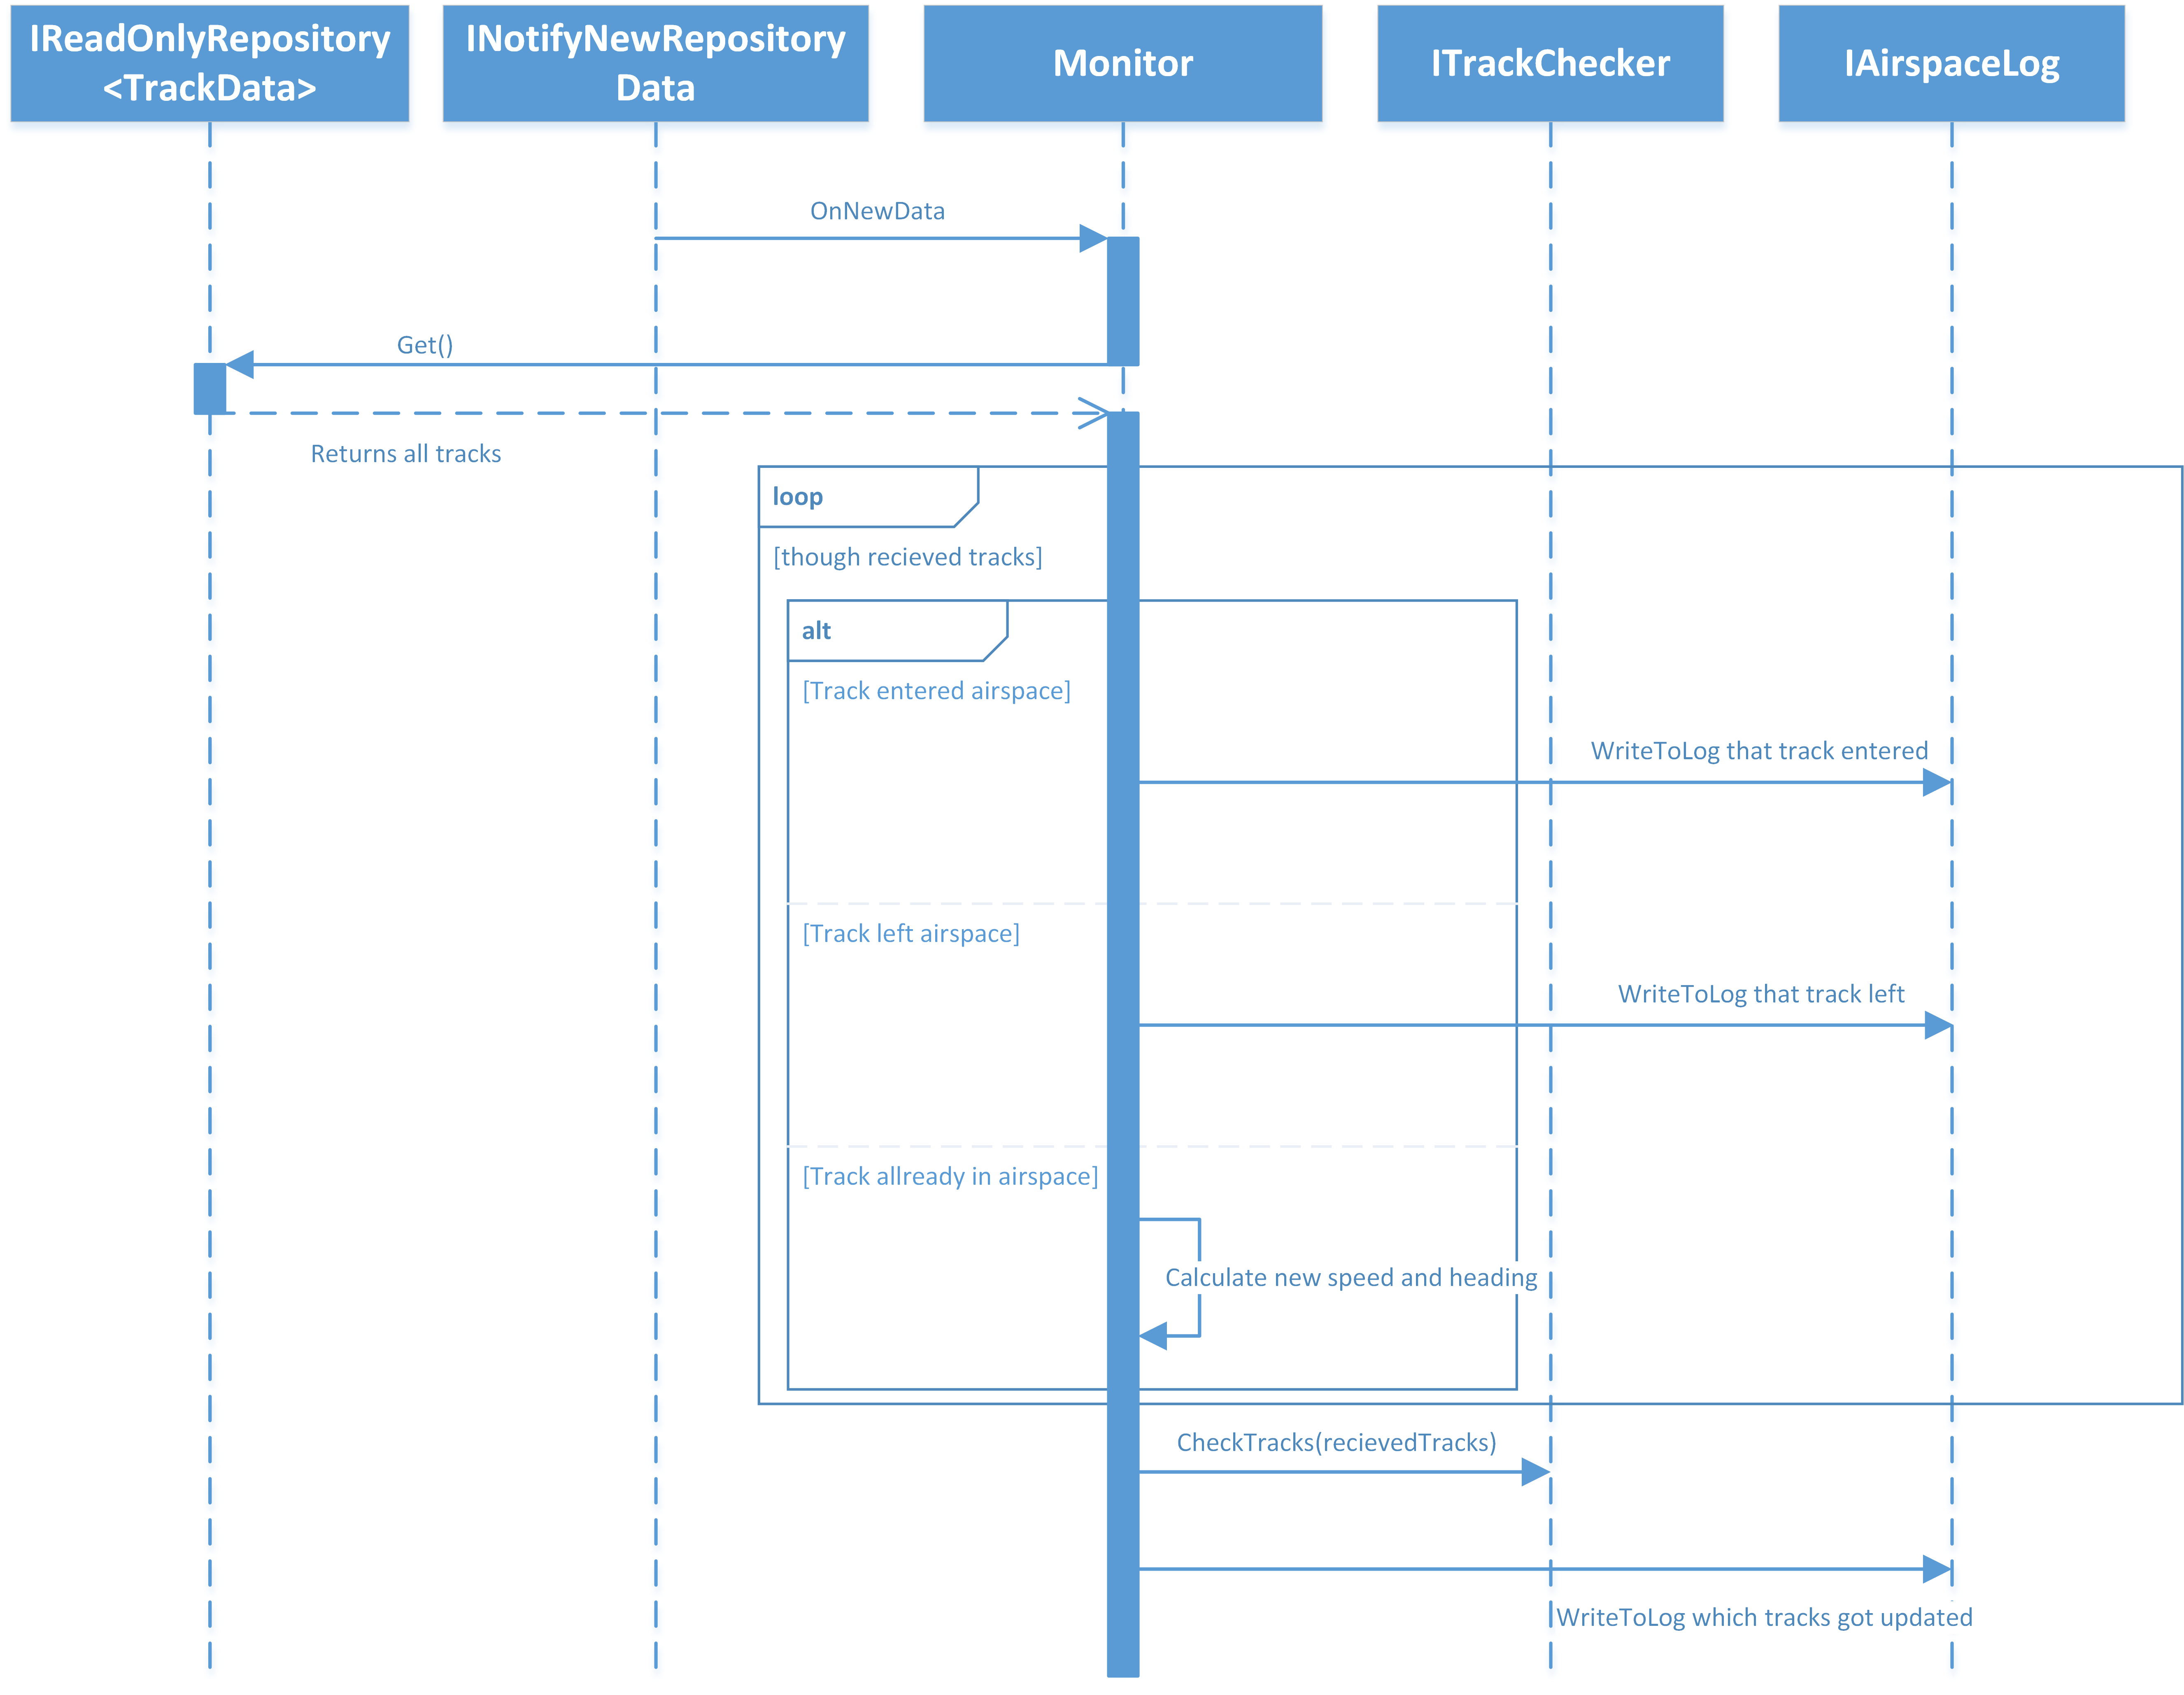
\includegraphics[width=1.0\linewidth]{Images/MonitorSeq}
	\caption{Sequence diagram for monitor}
	\label{fig:MonitorSeq}
\end{figure}

\begin{figure}
	\centering
	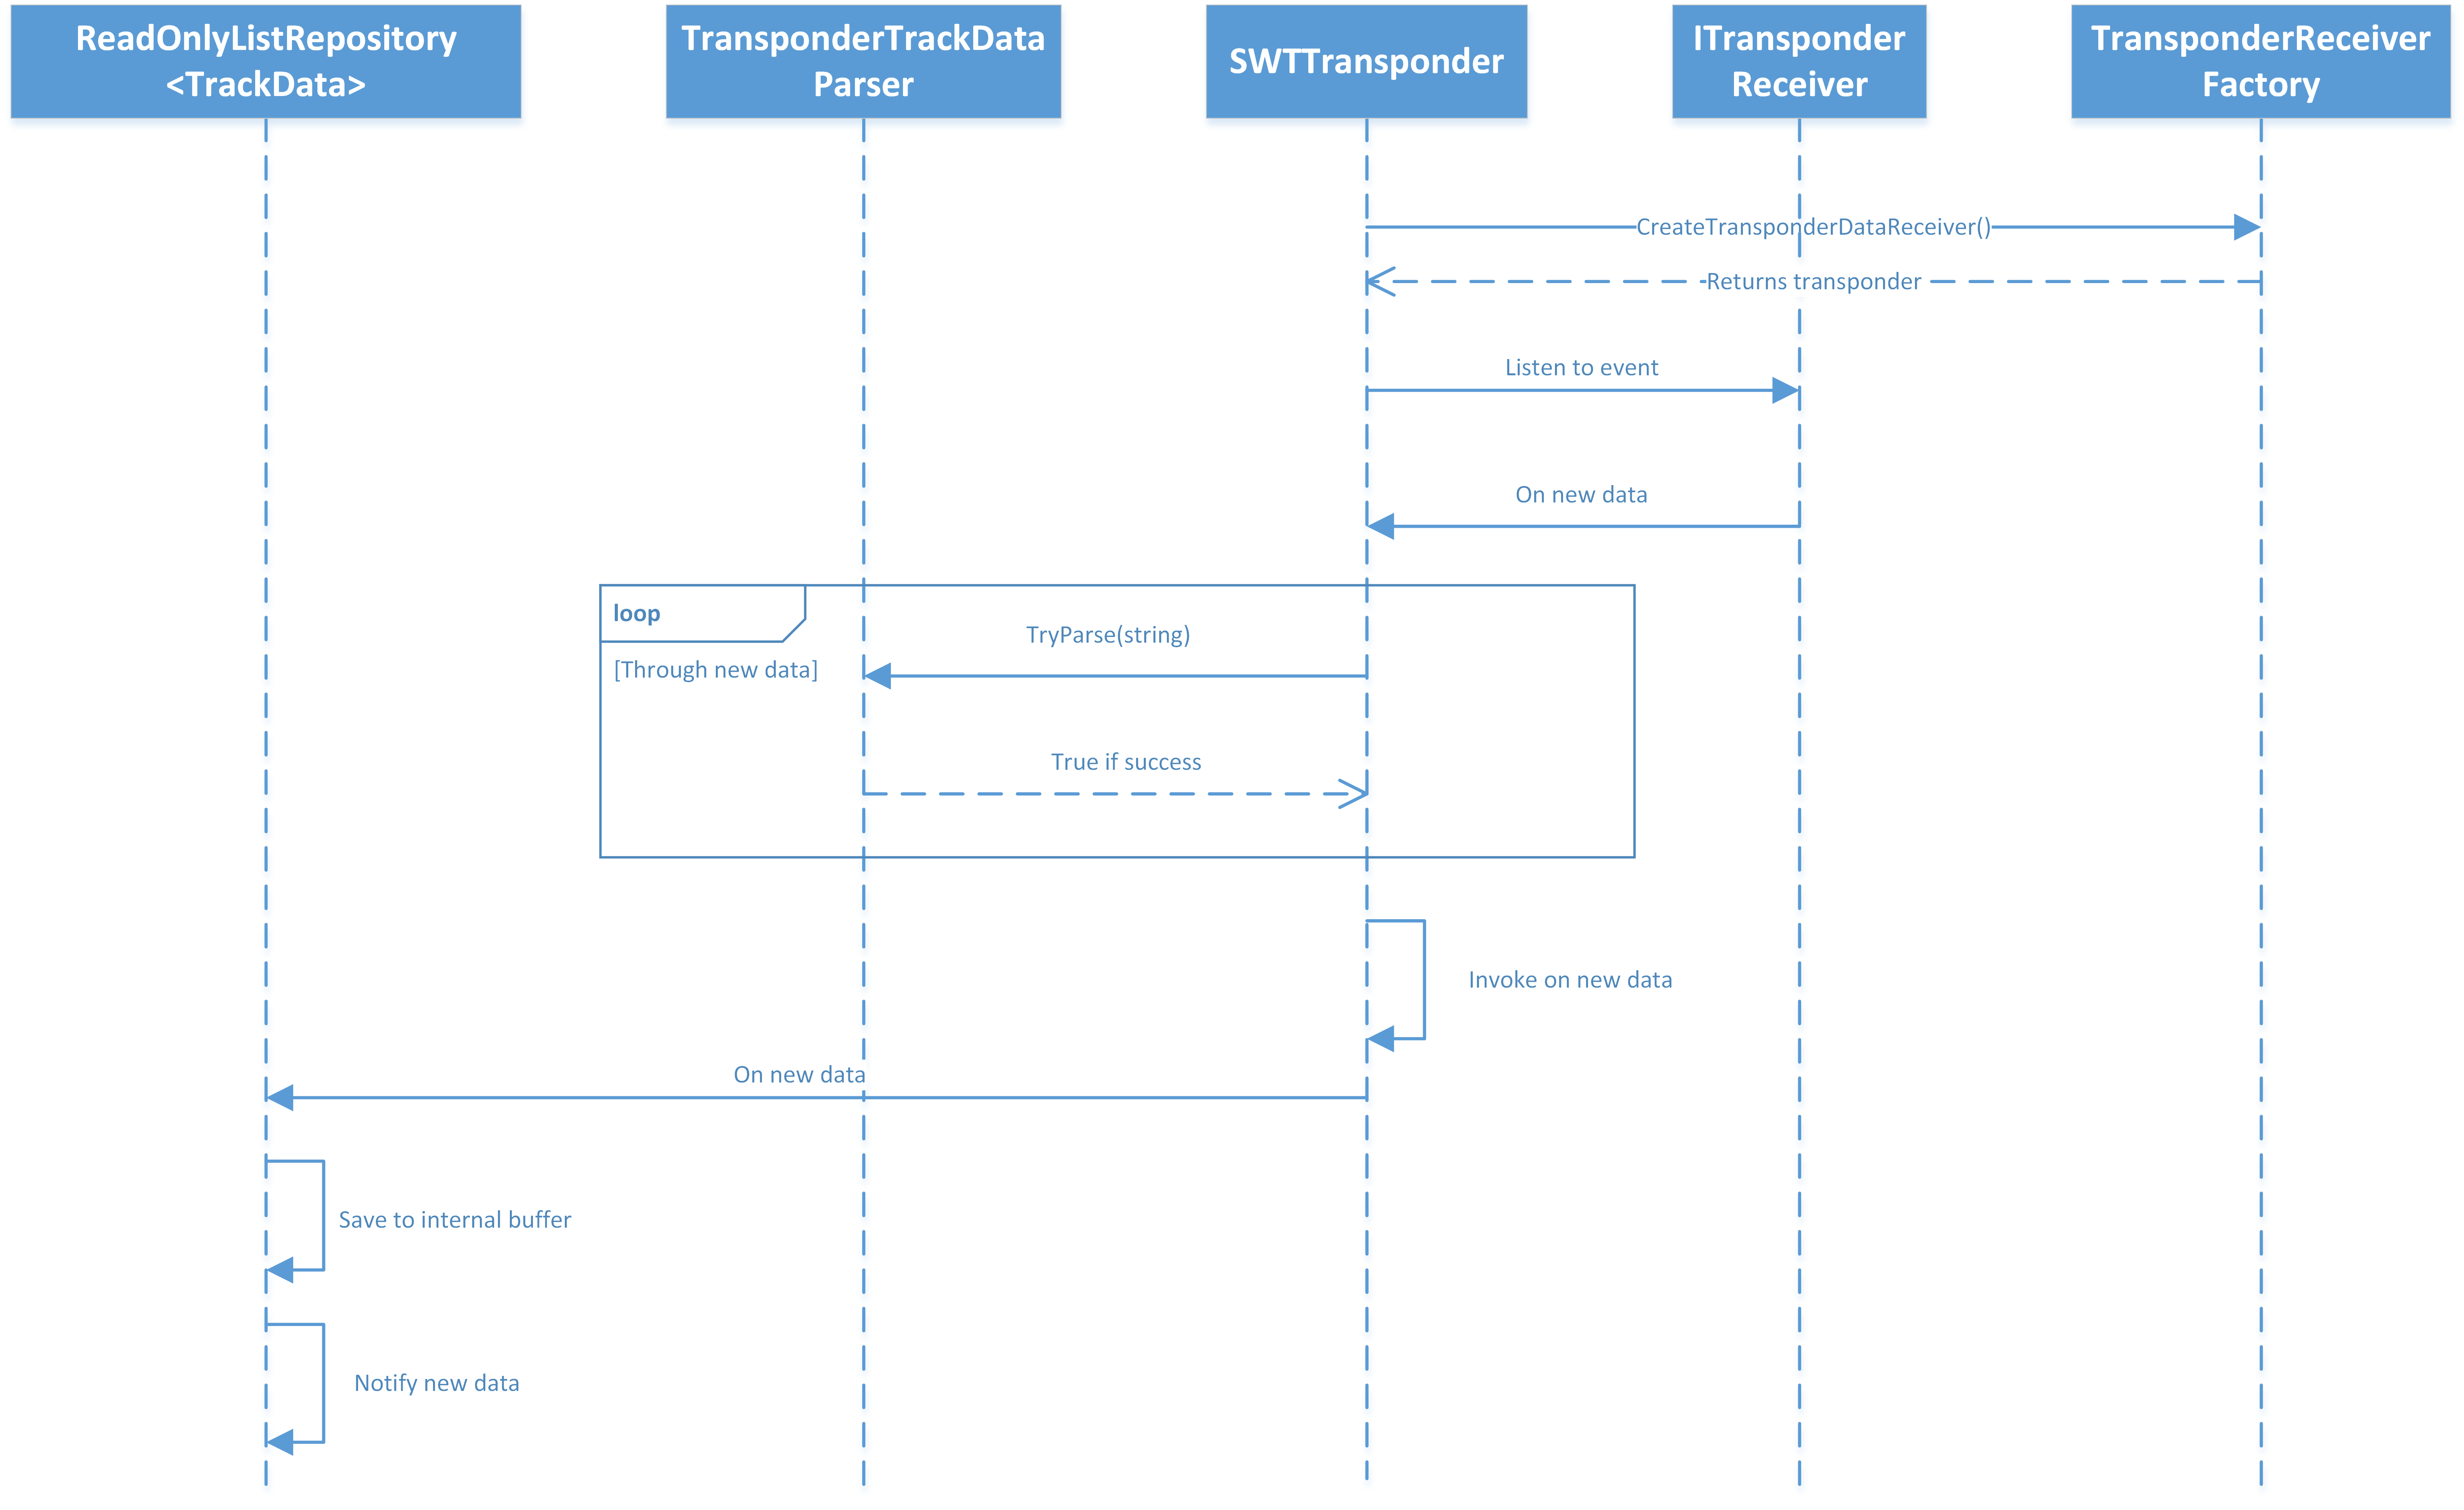
\includegraphics[width=1.0\linewidth]{Images/SWTTransponder}
	\caption{Sequence diagram for data acquisition from the transponder .DLL}
	\label{fig:SWTTransponderSeq}
\end{figure}

\subsection{Implementation}

It works

\begin{figure}
	\centering
	\includegraphics[width=1.0\linewidth]{"Images/Dependency tree"}
	\caption{Dependency tree}
	\label{fig:Dependencytree}
\end{figure}

\clearpage
